\section{The Usual, Spherical \Luscher's Formula}\label{sec:spherical}


Here we present a $D$-dimensional derivation of \Luscher's formula that roughly follows \Ref{Beane:2003da}, although the technology and sophistication of the finite-volume formalism has grown substantially \todo{cite cite cite}.  Assuming an interaction given by an tower of derivative contact operators
\begin{equation}
    V(p) = +\sum_n C_{2n}(\Lambda) p^{2n}
\end{equation}
where the interaction strengths depend on the regulator and carry spatial-dimension-dependent units.
The scattering amplitude is given by the bubble sum depicted in \Figref{bubbleSum}.

\begin{figure}[ht!]
\center
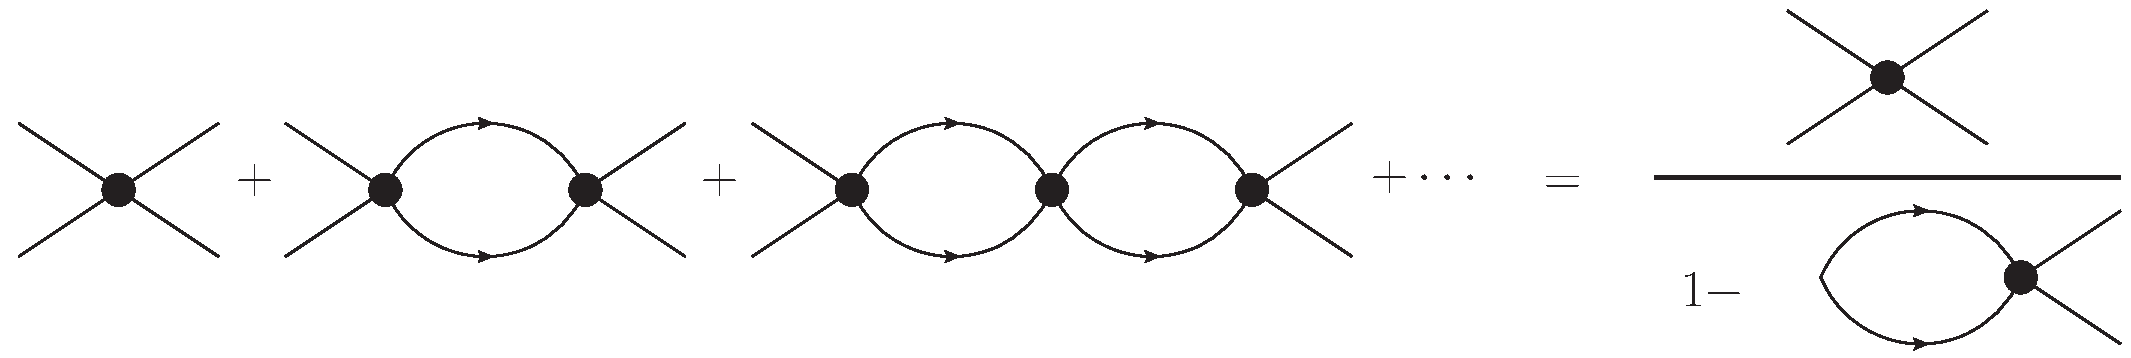
\includegraphics[width=.8\columnwidth]{figure/bubbleSum.pdf}
\caption{Bubble sum. Each line represents a propagator, each vertex represents $-i \sum_n C_{2n}(\Lambda) p^{2n}$, and the bubble is given by $I_0$ (see also \Figref{I0}).\label{fig:bubbleSum}}
\end{figure}

This bubble sum is a geometric series and gives, for the standard $T$-matrix, \cite{Kaplan:1998we,Beane:2003da}
\begin{equation}\label{eq:T matrix}
iT = \frac{-i\sum_n C_{2n}(\Lambda) p^{2n}}{1-I_0(p,\Lambda) \sum_n C_{2n}(\Lambda) p^{2n}},
\end{equation}
where $p$ is the relative momentum,  and $I_0(p,\Lambda)$ is a $D$-dependent function that arises from integrating the loop shown in \Figref{I0},
\begin{align}
    I_0(p)
    &=-i\int^{\Lambda/2}
        \frac { \mathrm {d}q_0}{2\pi}\ \frac{\mathrm { d } ^ { D } \vec{ q } } { (2\pi)^ { D } }
        \left( \frac { i } { \frac{E}{2} + q _ { 0 } - \frac{\vec{q}^2}{2m} + i \epsilon } \right)
        \left( \frac { i } { \frac{E}{2} - q _ { 0 } - \frac{\vec{q}^2}{2m} + i \epsilon } \right)
    \nonumber\\
    &=\frac{\Omega_D}{(2\pi)^D}\int^{\Lambda/2}  \mathrm { d } q \ q^{D-1}\left[\mathcal{P} \left( \frac { 1 } { E - \frac{\vec{q}^2}{m} } \right)
-i\frac{\pi m}{2q}\delta(q-\sqrt{mE})\right]
    \\
    &=\frac{\Omega_D}{(2\pi)^2}\frac{m}{L^{D-2}}\int^{\Lambda L/4\pi}  \mathrm { d } n \ n^{D-1}\left[\mathcal{P} \left( \frac { 1 } { \left(\frac{pL}{2\pi}\right)^2 - n^2 } \right)
-i\frac{\pi^2}{L n}\delta\left(\frac{2\pi}{L}n -p\right)\right]
    \label{eq:I0}
\end{align}
where $\mathcal{P}$ refers to Principle (Cauchy) Value, we have used the on-shell condition $mE=p^2$, and the geometric factor
\begin{equation}
\Omega_D=\frac{2\pi^{D/2}}{\Gamma(D/2)}=
    \begin{cases}
        4\pi    &   (D=3)\\
        2\pi    &   (D=2)\\
        2       &   (D=1)
    \end{cases}\ ,
\end{equation}

\begin{figure}[h!]
\center
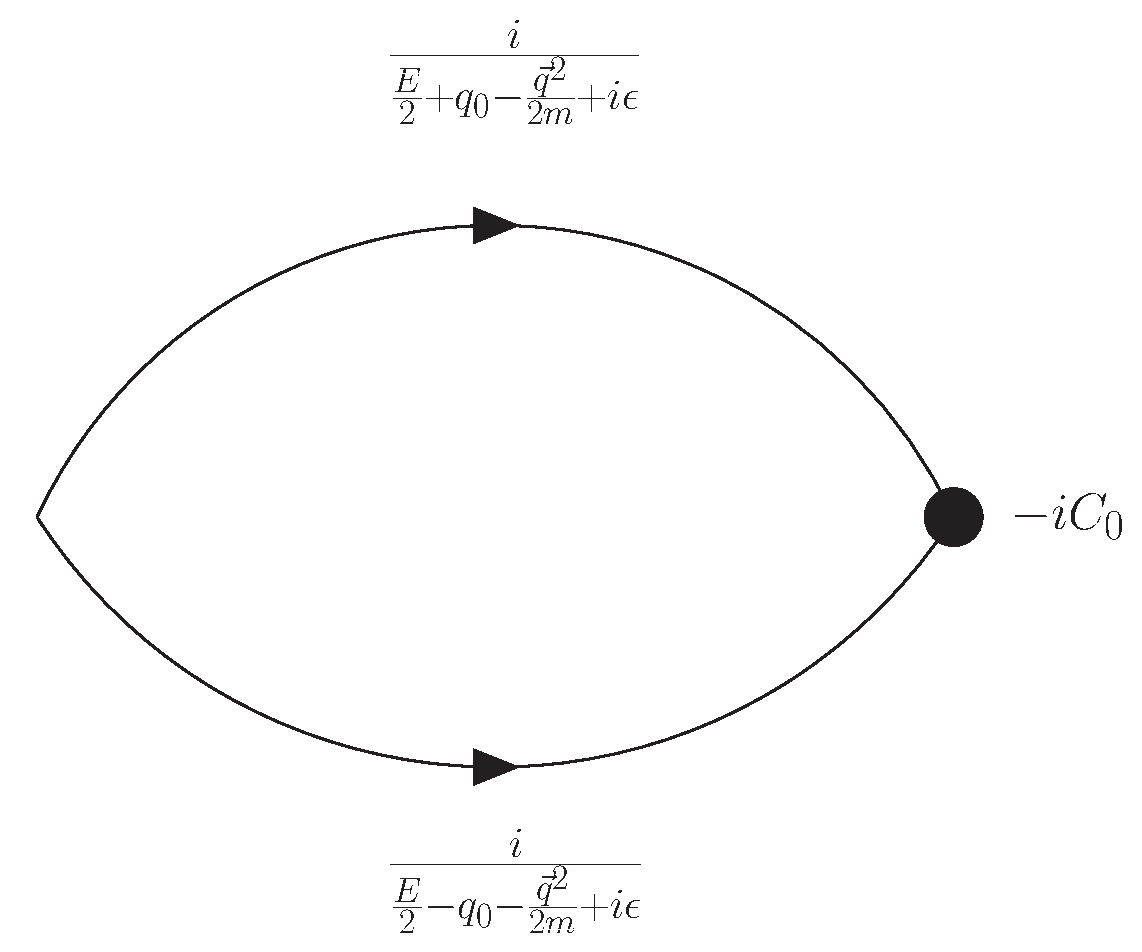
\includegraphics[width=.35\columnwidth]{figure/I0.eps}
\caption{Loop diagram contributing to $I_0$.\label{fig:I0} \todo{Make it a tower of interactions!  Also this figure is way too big cf the font.}}
\end{figure}

In the $s$-wave, the momentum-dependent $T$-matrix is related to the phase shift $\delta_0(p)$ by
\begin{equation}\label{eq:cot delta}
    i T = \frac{4}{m}\F_d\frac{i}{\cot \delta_0(p)-i}\ ,
\end{equation}
where
\begin{equation}
    \F_D
    =
    \begin{cases}
        \pi/p   & (D=3)\\
        1       & (D=2)\\
        p/2     & (D=1)
\end{cases}
\end{equation}
is a dimension-dependent kinematic factor.
This fixes the coefficients $C(\Lambda)$ as a function of the scattering data,
\begin{equation}\label{eq:IV pole}
    \frac{1}{\sum_n C_{2n}(\Lambda) p^{2n}}
    =
    I_0(p) - \frac{m}{4 \F_D}\left(\cot \delta_0(p) - i\right)
\end{equation}

In a finite volume, the energy eigenstates appear at poles of the $T$-matrix, so that
\begin{equation}\label{eq:FV pole}
    \frac{1}{\sum_n C_{2n}(\Lambda) p^{2n}} - I_{0,\FV}(p,L) = 0
\end{equation}
and the infinite-volume integral $I_0$ has been replaced by the matching finite-volume sum,
\begin{align}
I_{0,\FV}(p,L)
    &=-i\int \frac { \mathrm {d}q_0}{2\pi} \frac{1}{L^D}\sum_{\vec{q}}^{q < \Lambda/2} \left( \frac { i } { \frac{E}{2} + q _ { 0 } - \frac{\vec{q}^2}{2m} + i \epsilon } \right) \left( \frac { i } { \frac{E}{2} - q _ { 0 } - \frac{\vec{q}^2}{2m} + i \epsilon } \right)
    \\
    &=\frac{1}{L^D}\sum_{\vec{q}}^{q < \Lambda/2} \frac { 1 } { E - \frac{\vec{q}^2}{m} }
    =\frac{m}{(2\pi)^2 L^{D-2}} \sum_{\vec{n}}^{n < \frac{\Lambda L}{4\pi}} \frac{1}{x-n^2}
    &
    x &= \left( \frac{pL}{2\pi}\right)^2
\end{align}
where we have used the on-shell condition $mE=p^2$.  Combining the infinite-volume and finite-volume relations \eqref{IV pole} and \eqref{FV pole} yields
\begin{equation}
    \frac{m}{4\F_D}(\cot\delta_0(p)-i) = I_0(p) - I_{0,\FV}(p),
\end{equation}
the finite-volume quantization condition.

Plugging our results for the integrals in, one finds
\begin{equation}
    \frac{1}{4\F_D}\left(\cot \delta_0(p) - i\right) = \frac{1}{(2\pi)^2 L^{D-2}}\left[ \left(\int_{\vec{n}} - \sum_{\vec{n}}\right) \frac{1}{x-n^2} + \frac{-i \pi^2\Omega_D}{L} \int \mathrm{d}n\ n^{D-2} \delta\left(\frac{2\pi}{L}n - p\right) \right]
\end{equation}
where both the sum and integral are cut off by a restriction on the magnitude of $n$, $n^2 < (\Lambda L / 4\pi)^2$, and the integral implicitly carries a factor of $\Omega_D n^{D-1}$.
In a seemingly miraculous (but required) cancellation, the imaginary part on the left hand side exactly cancels the last term in the sum on the right, and we are left with
\begin{equation}
    p \cot \delta_0(p) = \frac{\F_D\ p}{\pi^2 L^{D-2}} \left(\sum_{\vec{n}}-\int_{\vec{n}}\right) \frac{1}{n^2-x}
\end{equation}
where $x=(pL/2\pi)^2$ and we switched the sign of the sum and integral as well as the sign of the denominator.
Because we cut off the sum and the integral in exactly the same way, in dimensions where $I_0$ diverges with $\Lambda$, the divergence cancels against the divergence in the sum.
Let $N=\Lambda L/2\pi$.
Then, defining, with a finite cutoff on magnitude $N/2$,
\begin{equation}\label{eq:spherical cutoff S}
    S^{\spherical N}_D(x) = \left(\sum_{\vec{n}}- \int_{\vec{n}}\right) \frac{1}{x-n^2}
\end{equation}
where the $\spherical$ superscript reminds us that we cut off our sum and integral in a spherical way, based on the magnitude of $n<N/2$, we recover the usual \Luscher zeta functions by taking
\begin{equation}
    S^\spherical_D(x)
    =
    \lim_{N\goesto\infty} S^{\spherical N}_D(x)
    =
    \lim_{N\rightarrow\infty}\left( \sum_{\vec{n}}^{n < N/2} \frac{1}{x-n^2} - \counterterm_D^\spherical \left(\frac{N}{2}\right)^{D-2}\right)
\end{equation}
where dimension-dependent counterterm $\counterterm_D^\spherical$ comes from the integral; we evaluate said counterterms in \Appref{counterterm/spherical}.
Finally,
\begin{equation}\label{eq:spherical quantization}
    p \cot \delta_0(p) = \frac{\F_D\ p}{\pi^2 L^{D-2}} S^\spherical_D(x).
\end{equation}
This is the usual \Luscher finite-volume quantization condition, and continuum-extrapolated energy levels should be fed through it to produce continuum-limit scattering data.
We have written it in such a way that the usual three-dimensional scattering quantity appear on the left-hand side but that is just a convenience, as we will discuss in \Secref{ere}.

\section{Matching, and the Effective Range Expansion}\label{sec:ere}

We can use the effective range expansion to express the scattering data as the sum of some known terms that do not vanish at low momentum and a series in $p^2$.  The expansion differs in different dimensions,
\begin{align}
    p\ (\cot \delta_0(p) - i)
    &=
    -\frac{1}{a} - ip + \frac{1}{2} r_0 p^2 \sum_j s_j (r_0^2 p^2)^j
    &
    (D&=3)
    \nonumber\\
    \cot \delta_0(p) - i
    &=
    \frac{2}{\pi} \log(a p) -i + \frac{1}{2} r_0^2 p^2 \sum_j s_j (r_0^2 p^2)^j
    &
    (D&=2)
    \\\nonumber
    \frac{\cot\delta_0(p)-i}{p}
    &=
    -\frac{i}{p} + a + \frac{1}{2} r_0^3 p^2 \sum_j s_j( r_0^2 p^2)^j
    &
    (D&=1)
\end{align}
where $a$ is the scattering length, $r_0$ the length scale called the effective range, and the $s_j$ are dimensionless shape parameters.
We can solve for the phase shift and encapsulate the low-energy pieces of the right-hand side into
\begin{equation}
    \lowEnergyA(p) =
    \begin{cases}
        -\frac{1}{ap}           &   (D=3)\\
        \frac{2}{\pi} \log ap   &   (D=2)\\
        ap                      &   (D=1)
    \end{cases}\ ,
\end{equation}
so that
\begin{equation}\label{eq:ERE}
    \cot \delta_0(p) - i = -i + \lowEnergyA(p) + \frac{1}{2} (r_0 p)^{4-D} \sum_j s_j \left(r_0^2p^2\right)^j.
\end{equation}
We can take this expression and plug it into \eqref{IV pole}, matching the dependence on $p$.
Using the spherical $I_0(p)$, one finds
\begin{align}
    \nonumber
    D&=3:
    &
    0&=\frac{4 \pi}{m C_0}-\frac{1}{a} + \frac{2N}{L}
    &
    0&=- \frac{4 \pi C_2}{m C_0^2} + \frac{1}{2}r_0 s_0 - \frac{2 L}{N \pi^2}
    &
    0&=\frac{4\pi(C_2^2-C_0 C_4)}{m C_0^3} + \frac{1}{2} r_0^3 s_1 - \frac{2L^3}{3\pi^4 N^3}
    &\ldots&
    \\
    D&=2:
    &
    0&=\frac{4}{m C_0} + \frac{2}{\pi} \log \frac{a N \pi}{L}
    &
    0&=- \frac{4 C_2}{m C_0^2} + \frac{1}{2}r_0^2 s_0  - \frac{L^2}{N^2 \pi^3}
    &
    0&=\frac{4(C_2^2-C_0 C_4)}{m C_0^3} + \frac{1}{2} r_0^4 s_1 - \frac{2 L^4}{4\pi^5 N^4}
    &\ldots&
    \\
    D&=1:
    &
    0&=\frac{2}{m C_0}+a-\frac{2L}{\pi^2N}
    &
    0&=- \frac{2 C_2}{m C_0^2} + \frac{1}{2}r_0^3 s_0 - \frac{2 L^3}{3N^3 \pi^4}
    &
    0&=\frac{2(C_2^2-C_0 C_4)}{m C_0^3} + \frac{1}{2} r_0^5 s_1 - \frac{2 L^5}{5\pi^6 N^5 }
    &\ldots&
    \nonumber
\end{align}
where $N/2$ is the cutoff on the integral, the first term in each relation comes from expanding $1/\sum_n C_{2n} p^{2n}$, the second from the effective range expansion \eqref{ERE}, and the third from expanding $I_0$ as a function of $p$, holding a fixed cutoff.  These equations can be solved order-by-order for the coefficients in the potential, or, if we know the coefficients, we can read these equations as determining the scattering data ($r_0$ and $s_j$) and how to correct for a finite cutoff.
\todo{Using $L=N\epsilon$ and $\epsilon=\pi/\Lambda$ I have checked that setting $C_{>0}=0$ reproduces 3-2-1-blastoff's (16), (17), (18) for D=3, (25) for D=2, and, when the cutoff is infinite, (28) for D=1.}

Of special note is the matching condition for $C_0$ when $D=2$, where the momentum dependence at small $p$ is logarithmic, and we cannot take an independent continuum and finite-volume limit.
\todo{What are we supposed again?  I used to understand this.  There's some dimensional transmutation magic going on here.}

We can also use this understanding to construct an improved \Luscher's formula.
Note that when passing from the cut off \eqref{spherical cutoff S} to \eqref{spherical S} we replaced the integral with its limiting value, the divergence-cancelling counterterm.
Rather than jump straight to the leading dependence on the cutoff, we can subtract subleading terms as well.
One finds, truncating our improvement scheme at order $J$,
\begin{align}
    S_3^\spherical(x)  = \lim_{N\goesto\infty} S^{\spherical N}_3(x)
    &=
    \lim_{N\goesto\infty}\left[\sum_{\vec{n}}^{n<N/2} \frac{1}{x-n^2}
        + 4\pi \sum_{j=0}^{J} \frac{x^j}{2j-1} \left(\frac{N}{2}\right)^{-(2j-1)}
    \right]
    &
    (D&=3)
    \\
    S_2^\spherical(x)  = \lim_{N\goesto\infty} S^{\spherical N}_2(x)
    &=
    \lim_{N\goesto\infty}\left[\sum_{\vec{n}}^{n<N/2} \frac{1}{x-n^2}
        + \pi \log \frac{x}{(N/2)^2}
        + \pi \sum_{j=1}^{J} \frac{x^j}{j} \left(\frac{N}{2}\right)^{-2j}
    \right]
    &
    (D&=2)
    \\
    S_1^\spherical(x)  = \lim_{N\goesto\infty} S^{\spherical N}_1(x)
    &=
    \lim_{N\goesto\infty}\left[\sum_{\vec{n}}^{n<N/2} \frac{1}{x-n^2}
        + 2 \sum_{j=0}^{J} \frac{x^j}{2j+1}\left(\frac{N}{2}\right)^{-(2j+1)}
        \right]
    &
    (D&=1)
\end{align}


\begin{center}
    \boxed{\textrm{{\color{red}REALLY TOUGH CHALLENGE: TELL THE ABOVE STORY WITH A CARTESIAN CUTOFF?}}}
\end{center}

\todo{I'm no longer convinced that (assuming you take the cutoff to infinity) spherical and cartesian should be different.  I think they should come out the same.}


\todo{STILL REMAINING:}
\begin{itemize}
    \item ERE / matching
    \item Describe tuning
    \item Show results in 2, 3D
    \item Something is wrong :(?  More like :D because we are smart!
\end{itemize}
